\chapter{Tail loss?}

\section{Introduction}


Chordates are composed of three subphyla\textemdash vertebra, urochordates and ephalochordate\textemdash that all share several characteristics, the notochord being the key characteristic, which is indicative of the phyla name. The tail development of larvacean (Oikopleura) and several species of ascidians, tunicates have been studied \cite{jeffery_factors_1992,nakatani_mutations_1999,kugler_evolutionary_2011}. Larvacean form tailed larvae with a hollow dorsal notochord and keep there tail throughout their adult life stage, ascidians do the same before undergoing the process of metamorphosis. A typical ascidian larvae tail forms through the convergence, intercalation and extension of the notochord \cite{swalla_mechanisms_1993}. When fully formed the ascidian notochord contains 40 cells, flanked by three rows of muscle. The ancestral notochord or notochord-like structure is believed to have been muscle based, this is perhaps the reason behind the tail formation being tied to both notochord and muscles \cite{lauri_development_2014}. This is not a far fetched idea seeing that the primary and secondary notochord and muscle lineage are derived from the same blastomere, and the ascidian tail needs both the notochord and differentiated muscle to form a larval tail \cite{nishida_cell_1987,di_gregorio_tail_2002}.

Of the \mytilde3000 species of ascidians less than 20 have been identified as undergoing tail-loss. Although each case of tail loss has happened independently, many of the ascidian that have undergone tail-loss tend to be Molgulide species \cite{berrill_studies_1931,huber_evolution_2000}. Although the mechanism behind tail-loss differs by species, a common characteristic is the lack of a notochord that intercalates and extends. \textit{M. bleizi} notochord cells converge to the midline, and began to extend, however, cells never properly intercalated and the tail formation stop before it is fully formed \cite{jeffery_evolution_1999}. In \textit{M. bleizi} there is an early down-regulation of \textit{bra}\textemdash a key notochord inducer\textemdash and muscle actin (\textit{MbMA}) has become pseudo genes.   

\textit{M. occulta} and \textit{M. oculata} are two closely related species, who in their adult form are virtually identical, with the exception of a white pigment spot between the two siphons of the tailed species, \textit{M. oculata}. During development the species are indistinguishable up to the gastrula stage. It is at late gastrula when the notochord and muscle cells begin to move posteriorly. There are several steps that take place to form the notochord and tail; first the notochord cells move mediolaterally to the midline, next the cells polarize and intercalate, changing their shape and extending posteriorly \cite{keller_mechanisms_2000, jiang_ascidian_2005,stemple_structure_2005}. This process is known as convergence and extension. 
genes necessary for tail formation that is missing from M. occulta has been found in other ascidians, for instance, macho-1 has been found the tail-less M. tectiformis. 
----
With advances in high throughput sequencing technologies, gene expression of M. occulta, M. oculata, and hybrid species can be analyzed \cite{gyoja_analysis_2007,pickrell_variation_2010}. The transcriptomes of three different developmental stages of M. occulta, M. oculata, and hybrids have been sequenced at Michigan State University. The three transcriptomes were used to identify the presence or absence of known notochord genes downstream of bra using C. intestinalis data from the NCBI database. BLAST searches were with known notochord genes, and several of them were selected for further analysis. FGF9/16/20, prickle (pk), and several other downstream brachyury factors?noto6, leprecan, merlin, and noto17?were analyzed for presence, temporal and spatial expression using in situ hybridizations. In addition to focusing on the notochord genes an EdgeR differential expression analysis was done to identify other genes that are involved in tail development.

Simple body plan with a small number of cells \cite{satoh_ascidian_2001,satoh_genome_2002}, rapid embryo development.

Induced at the 32 cell stage by \textit{FGF9/16/20}
muscle and notochord come from the same cell lineage.
Hybrids are tails are resorted in embryos that contain p58, which stains in the muscle 
It is thought that the early form of the notochord where not cartilage based but were made of muscle.   
----
\section{Methods}
\subsection{Sample collection, sequencing and assembly}
DNA was extracted from the gonads of an individual adult specimen for M. occidentalis, M. occulta, and M. oculata. Paired in jumping libraries were collected for each sample ranging from \mytilde300bp to \mytilde950bp. further details about extraction methods and libraries can be found in Stolfi et al., \cite{}. RNA was extracted from all three molgula species using the methods discussed in Lowe et al., \cite{}. Sequencing for M. occulta and M. oculata was conducted at the Michigan State University 



Genome assembly was conducted using 3-pass digital normalization\cite{} and assembled using Velvet\cite{}. Assemblies were done with 21 
Both de novo and reference based assembly were used when creating gene models. 
reads were mapped to their respective genomes using bra and top hat to identify genes and alternative splicing variants. the accepted.bam hits ere then sorted and indexed using samtools. the sorted bam files where then processed using cufflinks and cuff merge to generated consenus gtf annotation files. the de novo assembled transcripts from Lowe et al., were aligned to their respective genomes using BLAT. the cufflinks/cuffmerged gtf files were then covered into bed file and the read mapped annotation and de novo assembled aligned annotation files were merged using gimme. Gimme joins gene models using a graph based method to develop more complete transcripts. the gimme gene models were then covertedd to gff format using the crript bed2gff in the gimme utils folder in order to extract the transcripts from the genome in a multi pasta file. transcripts were then partitioned into transcript families using khmer partitioning tool. 

\subsection{Gene counts and differential expression analysis}
reads are mapped to transcripts from the gimme gene modules for their respective species. Hybrid reads are mapped onto the M. occulta and M. oculata genomes as well, seeing that they are F1 hybrids and should contain an allele from each parent. Read counts were generated using express \cite{}. Effective counts, which normalizes counts based on transcript length were used because transcript length will differ across species. A replicate was only provided for one of the samples, 3hpf, because of this various dispersion calculation methods were used. the one replicate was used to calculated statistics, in addition to 5hpf being treated as a replicate for 6hpf. These time points represent what would be early and mid-tail bud stages in the urodele ascidian. 

Notochord genes have been identified using subtractive hybridization, mircoarrays and 

\section{Results}
\subsection{\textit{M. occulta} and \textit{M. oculata} have strong overlap in gene presence}
\textit{C. intestinalis} is the closest ascidian species with a well annotated gene, because of these reason it was used to annotate the genomes of both \textit{M. occulta} and \textit{M. oculata}. 

-----
\subsection{Notochord gene network}

Reciprocal best hit (RBH) blast with an e-value of 1e-6, were done with the M. occulta and M. oculata transcriptomes against C. intestinalis for the annotation of each species. M. occulta and M. oculata have a high overlap in number of translated transcripts that showed homology with C. intestinalis proteins from the NCBI database. Of the 16 thousand proteins found in the NCBI database, both molgulid species recovered  ~84\% of the proteins. M. occulta had an additional 202 transcripts that were not found in M. oculata and M. oculata had an additional 250 transcripts that did not have hits in M. occulta, overlapping by 97\%. Next, we examined genes associated with notochord development in C. intestinalis to better analyze the molecular development of the tail.  Seventy-two genes identified as being involved in notochord development (Kugler et al 2008; Hotta et al 2000; Kugler et al. 2011; Jose?-Edwards 2011) were BLAST against each species. Four genes?not1, not4, not5, and snail?were not found in either of the species. This could have been due to true absence or sequence divergence in the transcripts. The remaining 68 genes were shared by both species with the exception of col5a, which was missing from M. occulta. Several genes found in the Ciona notochord GRN were not discovered in either M. occulta or M. oculata. Noto1, noto5, noto14, noto16, and ... were all missing from the transcriptomes of M. occulta and M. oculata. Additionally Kihf5 was not found in M. oculata but showed homology in M. occulta. M. occulta did not have 3 genes that were found in M. oculata, netrin, noto9 and something. 

\begin{figure}[tbp]
\centering
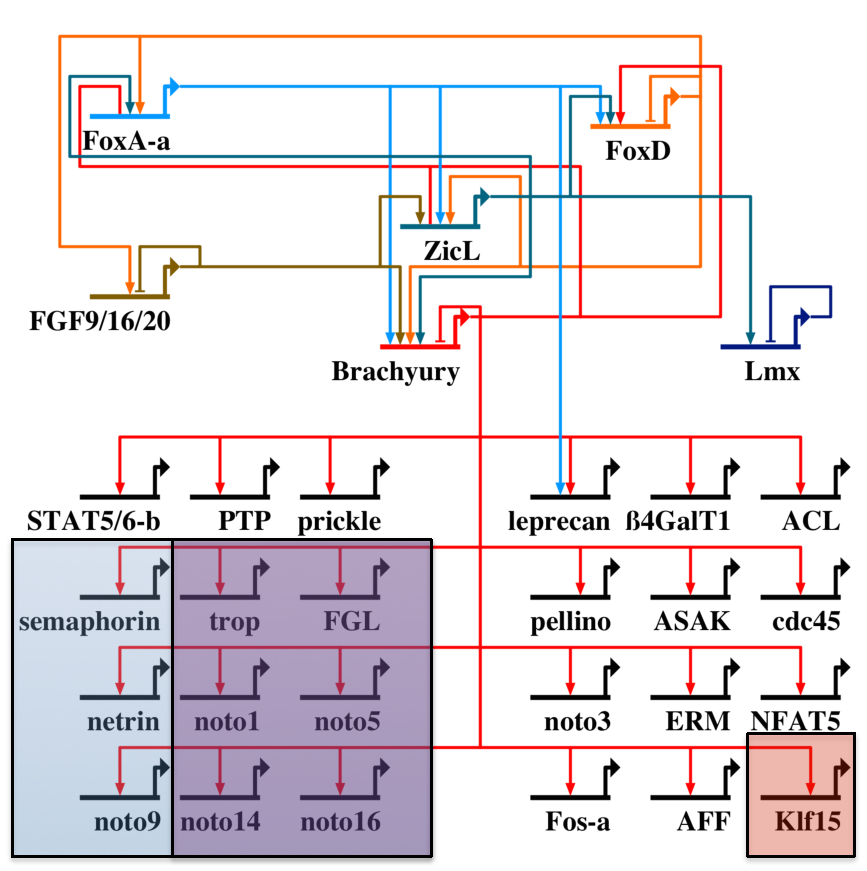
\includegraphics[scale=0.55]{figures/bra_grn.pdf}
\caption{\textbf{Hox cluster for \textit{Hox 10, 12-13} in \textit{M. occulta}, \textit{M. oculata} and \textit{M. occidentalis}} }
\label{fig:hox12}
\end{figure}

\begin{figure}[tbp]
\centering
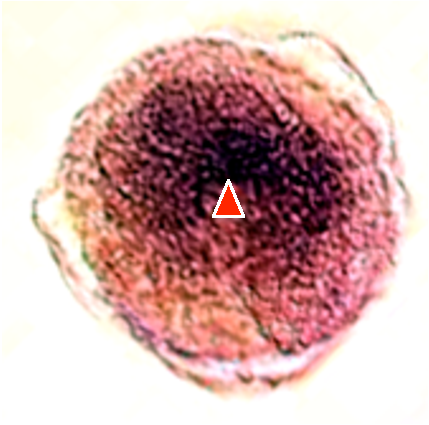
\includegraphics[scale=0.55]{figures/prickle.pdf}
\caption{\textbf{Hox cluster for \textit{Hox 10, 12-13} in \textit{M. occulta}, \textit{M. oculata} and \textit{M. occidentalis}} }
\label{fig:hox12}
\end{figure}



\subsection{Prelliminary results: EdgeR differential expression analysis by stage} 

Gene expression at the gastrula stage does not show a great deal of fold-change between M. occulta, M. oculata and the hybrid. The majority of the genes had a fold-change of less than 5 fold, and most of the genes clustered inside of that 5-fold window (Figure 3a).  The fact that the majority of the genes do not show significant fold-change is not surprising because M. occulta and M. oculata are very similar at this stage of development (Swalla and Jeffery 1990).  When comparing each species to the hybrid, most of the genes clustered within a 5-fold-change window. 
During neurulation M. occulta versus M. oculata differential expression pattern is similar to gastrula stage, clustering within a 5 fold-change window. However, there is a drastic different in the fact that ~300 of the genes have a 10 fold-change in expression (Figure 3d).  The change in expression between the two species mirrors what was observed in morphological studies (Swalla and Jeffery 1990). M. occulta has normal urodele?tailed?development up to gastrula and begins to diverge at neurulation. Of the genes that were higher expressed in M. oculata compared to M. occulta, those same genes were higher expressed in hybrids versus M. occulta. Those genes do not show significant differential expression when comparing M. oculata to hybrid. There are ~20 transcripts that show a 10 fold-change increase in expression in hybrid compared to M. oculata.
